\documentclass[a4paper, 12pt]{article}
\usepackage{amsthm, amsmath, amssymb}
\usepackage[margin=1in, a4paper]{geometry}
\usepackage{tikz}
% \usepackage{pgfplots}

\usetikzlibrary{patterns,arrows.meta}

\title{Dirichlet's Hyperbolic Method}
\author{}
\date{}

\newtheorem{thm}{Theorem}
\newtheorem{cor}{Corollary}

\begin{document}
\maketitle

\begin{thm}[Dirichlet's Hyperbolic Method]
Let $f, g$ be two arithmetic functions. Let $S_{f}(x)$ and $S_g(x)$ be the summatory functions of $f$ and $g$ respectively. For any real number $x\ge1$ and any parameter $1 \le y \le x$, then
$$
    S_{f*g}(x) = \sum_{n\le x}(f*g)(n)
$$
$$
    = \sum_{n\le y}f(n)S_{g}\left(\frac{x}{n}\right) + \sum_{m\le\frac{x}{y}}g(m)S_{f}\left(\frac{x}{m}\right) - S_{f}(y)S_{g}\left(\frac{x}{y}\right)
$$
\end{thm}

\begin{proof}
\begin{align*}
    S_{f*g}(x)
    &= \sum_{n\le x}(f*g)(n) \\
    &= \sum_{n\le x}\sum_{md=n}f(m)g(d) = \sum_{md\le x}f(m)g(d)
\end{align*}

The condition $md\le x$ defines a region in the 1st quadrant $m,d$ plane bounded by $d=\frac{x}{m}$.

\begin{figure}[ht]
\centering
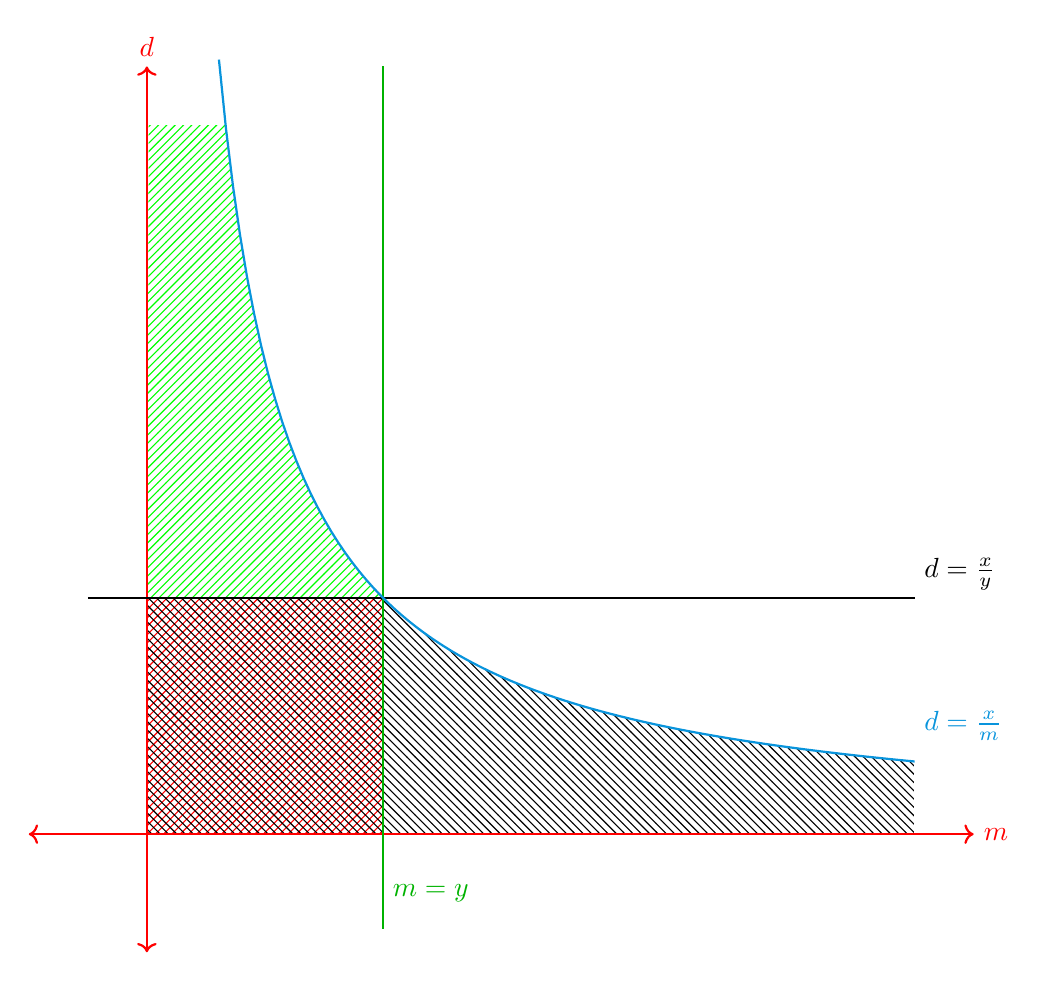
\begin{tikzpicture}[xscale=1.5, yscale=1.5]

    \begin{scope}
        \fill[pattern=north east lines, pattern color=red] (0,0) rectangle (2,2);
        \fill[pattern=north west lines, pattern color=black] (0,0) rectangle (2,2);

        \begin{scope}
            \clip (0,2) rectangle (2,6);
            \fill[pattern=north east lines, pattern color=green]
                (0,0) -- plot[domain=0.1:2, samples=100] (\x, {4/\x}) -- (2,0) -- cycle;
        \end{scope}

        \begin{scope}
            \clip (2,0) rectangle (6.5,2);
            \fill[pattern=north west lines, pattern color=black]
                (2,0) -- plot[domain=2:6.5, samples=100] (\x, {4/\x}) -- (6.5,0) -- cycle;
        \end{scope}
    \end{scope}

    \draw[<->, thick, red] (-1, 0) -- (7, 0) node[right] {$m$};
    \draw[<->, thick, red] (0, -1) -- (0, 6.5) node[above] {$d$};

    \draw[thick, black] (-0.5, 2) -- (6.5, 2);
    \node[ right] at (6.5, 2.2) {$d=\frac{x}{y}$};

    \draw[thick, green!70!black] (2, -0.8) -- (2, 6.5);
    \node[green!70!black, right] at (2, -0.5) {$m=y$};

    \draw[thick, cyan!80!blue, domain=0.61:6.5, samples=100] plot (\x, {4/\x});

    \node[cyan!80!blue, right] at (6.5, 4/6.5 + 0.3) {$d = \frac{x}{m}$};

\end{tikzpicture}

\caption{Geometric interpretation of the Dirichlet hyperbola method.}
\end{figure}

\noindent Region A: $m \le y, d \le \frac{x}{m}$ \\
Region B: $d \le \frac{x}{y}, m \le \frac{x}{d}$ \\
Region C: $m \le y, d \le \frac{x}{y}$

\vspace{1em}
\noindent \textbf{- Sum over A} \\
\begin{align*}
    \Sigma_{A} &= \sum_{m\le y}\sum_{d\le\frac{x}{m}}f(m)g(d) \\
    &= \sum_{m\le y}f(m)\sum_{d\le\frac{x}{m}}g(d) = \sum_{m\le y}f(m)S_{g}\left(\frac{x}{m}\right)
\end{align*}

\noindent \textbf{- Sum Over B:} \\
\begin{align*}
    \Sigma_{B} &= \sum_{d\le\frac{x}{y}}\sum_{m\le\frac{x}{d}}f(m)g(d) \\
    &= \sum_{d\le\frac{x}{y}}g(d)\sum_{m\le\frac{x}{d}}f(m) = \sum_{d\le\frac{x}{y}}g(d)S_{f}\left(\frac{x}{d}\right)
\end{align*}

\noindent \textbf{- Sum Over C} \\
\begin{equation*}
    \Sigma_{C} = \sum_{m\le y}f(m)\sum_{d\le\frac{x}{y}}g(d) = S_{f}(y)S_{g}\left(\frac{x}{y}\right)
\end{equation*}

Now collecting and substracting the region C (since it was counted twice), we get:
$$
    S_{f*g}(x) = \sum_{n\le y}f(n)S_{g}\left(\frac{x}{n}\right) + \sum_{m\le\frac{x}{y}}g(m)S_{f}\left(\frac{x}{m}\right) - S_{f}(y)S_{g}\left(\frac{x}{y}\right)
$$
\end{proof}

\begin{cor}[Lowest Error] Taking $y = \sqrt{x}$ in the previous theorem gives the lowest error (best approximation).
\begin{equation*}
    \sum_{n\le x}(f*g)(n) = \sum_{n\le\sqrt{x}}f(n)S_{g}\left(\frac{x}{n}\right) + \sum_{n\le\sqrt{x}}g(n)S_{f}\left(\frac{x}{n}\right) - S_{f}(\sqrt{x})S_{g}(\sqrt{x})
\end{equation*}
\end{cor}


\begin{cor}[$y=1$]
\begin{align*}
    S_{f*g}(x) &= \sum_{n\le 1}f(n)S_{g}\left(\frac{x}{n}\right) + \sum_{m\le x}g(m)S_{f}\left(\frac{x}{m}\right) - f(1)S_{g}(x) \\
    &= f(1)S_{g}(x) + \sum_{m\le x}g(m)S_{f}\left(\frac{x}{m}\right) - f(1)S_{g}(x) \\
    &= \sum_{m\le x}g(m)S_{f}\left(\frac{x}{m}\right)
\end{align*}
\end{cor}

\end{document}
